% Options for packages loaded elsewhere
\PassOptionsToPackage{unicode}{hyperref}
\PassOptionsToPackage{hyphens}{url}
%
\documentclass[
]{book}
\usepackage{amsmath,amssymb}
\usepackage{iftex}
\ifPDFTeX
  \usepackage[T1]{fontenc}
  \usepackage[utf8]{inputenc}
  \usepackage{textcomp} % provide euro and other symbols
\else % if luatex or xetex
  \usepackage{unicode-math} % this also loads fontspec
  \defaultfontfeatures{Scale=MatchLowercase}
  \defaultfontfeatures[\rmfamily]{Ligatures=TeX,Scale=1}
\fi
\usepackage{lmodern}
\ifPDFTeX\else
  % xetex/luatex font selection
\fi
% Use upquote if available, for straight quotes in verbatim environments
\IfFileExists{upquote.sty}{\usepackage{upquote}}{}
\IfFileExists{microtype.sty}{% use microtype if available
  \usepackage[]{microtype}
  \UseMicrotypeSet[protrusion]{basicmath} % disable protrusion for tt fonts
}{}
\makeatletter
\@ifundefined{KOMAClassName}{% if non-KOMA class
  \IfFileExists{parskip.sty}{%
    \usepackage{parskip}
  }{% else
    \setlength{\parindent}{0pt}
    \setlength{\parskip}{6pt plus 2pt minus 1pt}}
}{% if KOMA class
  \KOMAoptions{parskip=half}}
\makeatother
\usepackage{xcolor}
\usepackage{longtable,booktabs,array}
\usepackage{calc} % for calculating minipage widths
% Correct order of tables after \paragraph or \subparagraph
\usepackage{etoolbox}
\makeatletter
\patchcmd\longtable{\par}{\if@noskipsec\mbox{}\fi\par}{}{}
\makeatother
% Allow footnotes in longtable head/foot
\IfFileExists{footnotehyper.sty}{\usepackage{footnotehyper}}{\usepackage{footnote}}
\makesavenoteenv{longtable}
\usepackage{graphicx}
\makeatletter
\def\maxwidth{\ifdim\Gin@nat@width>\linewidth\linewidth\else\Gin@nat@width\fi}
\def\maxheight{\ifdim\Gin@nat@height>\textheight\textheight\else\Gin@nat@height\fi}
\makeatother
% Scale images if necessary, so that they will not overflow the page
% margins by default, and it is still possible to overwrite the defaults
% using explicit options in \includegraphics[width, height, ...]{}
\setkeys{Gin}{width=\maxwidth,height=\maxheight,keepaspectratio}
% Set default figure placement to htbp
\makeatletter
\def\fps@figure{htbp}
\makeatother
\setlength{\emergencystretch}{3em} % prevent overfull lines
\providecommand{\tightlist}{%
  \setlength{\itemsep}{0pt}\setlength{\parskip}{0pt}}
\setcounter{secnumdepth}{5}
\ifLuaTeX
  \usepackage{selnolig}  % disable illegal ligatures
\fi
\usepackage[]{natbib}
\bibliographystyle{apalike}
\usepackage{bookmark}
\IfFileExists{xurl.sty}{\usepackage{xurl}}{} % add URL line breaks if available
\urlstyle{same}
\hypersetup{
  pdftitle={Study Note for 24Q2 AppFin704},
  pdfauthor={Author: Jung Xue},
  hidelinks,
  pdfcreator={LaTeX via pandoc}}

\title{Study Note for 24Q2 AppFin704}
\author{Author: Jung Xue}
\date{Last Updated: 2024-05-26}

\begin{document}
\maketitle

{
\setcounter{tocdepth}{1}
\tableofcontents
}
\chapter{Investments and Securities Markets}\label{ch1}

•describe differences among asset classes and construction of stock market indexes, and calculate profit/loss on options/futures investments.

•describe how firms issue securities, and identify types of investors' orders

•compare mechanics and implications of buying on margin \& short selling

•cite pros/cons of investing with an investment company, and contrast open end mutual funds with other types of investment companies.

•define net asset value (NAV) and measure the rate of return on a mutual fund, and classify mutual funds according to investment style.

•demonstrate the impact of expenses and turnover on fund performance

\section{Asset Classes and Financial Instruments}\label{asset-classes-and-financial-instruments}

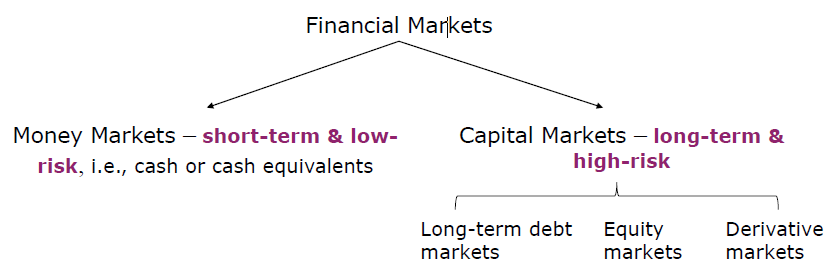
\includegraphics{Resources/Financialmarkets.png}

\subsection{Money Markets}\label{money-markets}

\begin{itemize}
\tightlist
\item
  Treasury bills
\item
  Certificates of Deposits (Term Deposits)
\item
  Commercial Paper(CP) (short term \textless{} 12month unsecured debts)
\item
  Bankers Acceptances (a postdated check, A bank, rather than an account holder, guarantees the payment.)
\item
  Eurodollars (U.S. dollar denominated deposits at foreign banks or foreign branches of U.S. banks)
\item
  Repurchase Agreements (Repos or RPs) and Reverse Repos.
\item
  Others, e.g., Brokers' Calls (interests charged by banks on loans made to brokerage firms), Federal Funds, The LIBOR Market, and Money Market Funds
\end{itemize}

\subsection{The Bond Market}\label{the-bond-market}

\begin{itemize}
\tightlist
\item
  Treasury Notes/Bonds (\$21 billion, \$21/\$51= 41\% of 2020 US Bond Market)
\item
  Mortgages and Mortgage Backed Securities (\$12.7 billion, 25\%
\item
  Corporate Bonds, including secured bonds, debentures (unsecured), callable/puttable/convertible bonds (\$10.6 billion, 21\%
\item
  Municipal Bonds (Issued by states/local, tax exempt) (\$3.95 billion, 7.8\%)
\item
  Federal Agency Debt, e.g., Fannie Mae, Freddie Mac ( 3.3\%)
\item
  International Bonds

  \begin{itemize}
  \tightlist
  \item
    Eurobonds: Eurodollar bonds bonds denominated in a currency other than the issuer's currency
  \item
    Yankee bond: US dollar denominated bond sold in the U.S. by a non U.S. issuer
  \end{itemize}
\item
  Inflation Protected Bonds (i.e., principal is adjusted per CPI)
\end{itemize}

\subsection{The Equity Market}\label{the-equity-market}

\begin{itemize}
\tightlist
\item
  Common stocks
\item
  Preferred stocks (pay preferred dividends, behaving like bond)
\item
  Depository receipts, (shares in a foreign company)

  \begin{itemize}
  \tightlist
  \item
    ADR American Depository Receipt
  \item
    CRD Chinese Depository receipt
  \item
    Reduced currency and foreign operation cost
  \end{itemize}
\end{itemize}

\subsection{Stock and bond market indexes}\label{stock-and-bond-market-indexes}

\begin{itemize}
\tightlist
\item
  Broad based index (S\&P 500 etc.)
\item
  Narrow based index (composed of only a few stocks, in a specific industry)
\item
  Why indexes?
\item
  Provide performance benchmarks
\item
  Base of derivatives
\item
  Smart beta
\end{itemize}

The goal of \textbf{Smart beta} is to obtain alpha, lower risk or increase diversification at a cost lower than traditional active management and marginally higher than straight index investing

Construction Methodology

\begin{itemize}
\tightlist
\item
  Price weighted (DJIA) 1 share per firm
\item
  Market value weighted (S\&P500, NASDAQ)
\item
  Equal weighted (simple average of returns)
\end{itemize}

\subsection{Derivative Markets}\label{derivative-markets}

\begin{itemize}
\tightlist
\item
  A security with a pay-off that depends on the prices of other securities
\item
  Call/put options
\item
  Futures/Forwards
\item
  Swaps, futures options, etc.
\end{itemize}

Why we need them?

\begin{itemize}
\tightlist
\item
  Speculative
\item
  Hedging
\item
  Arbitraging (to lock in price)
\end{itemize}

\textbf{Arbitrage} describes the act of buying a security in one market and simultaneously selling it in another market at a higher price, thereby enabling investors to profit from the temporary difference in cost per share.

\section{Securities Markets and Trading}\label{securities-markets-and-trading}

Originators

\begin{itemize}
\tightlist
\item
  Publicly traded companies initial public offering (IPO), and seasonal equity offerings (SEOs), - Privately held firms (private placement in which shares are sold directly to
  a small group of institutional or wealthy investors)
\item
  Shelf registrations (public firms can register securities and gradually sell them to the public )
\end{itemize}

How securities are traded (in secondary markets)

\begin{itemize}
\tightlist
\item
  Direct search (e.g.~painting)
\item
  Brokered
\item
  Dealer
\item
  Auctions
\end{itemize}

ype of orders
maket order
price contingeant order

Trading mechanisms
OTC dealer
electronic
market maker (increase liquidity)
--
Over the counter dealer markets (OTC Markets)
-
Electronic communication networks ( ECNs)

margin trading

why to purchase with margin?

able to make more profits by borrowing money from broker, essentially multiplying market fluctuation/volatility.

short sale (borrow stocks to sell and payback when you sold it at profit)

derivative market (sell, not borrowing)

\section{Market Participants}\label{market-participants}

\subsection{Investment company}\label{investment-company}

\begin{itemize}
\tightlist
\item
  Intermediary that invest for investors
\item
  Record and admin
\item
  professional management
\item
  Lower transaction cost by volume
\end{itemize}

Net Asset Value (NAV)

\[\frac{Asset - Liabilities}{share outstanding}\]
unit investement fund (unmanaged) fixed portfolio for life

Managed Investment companies
- open-end(publicly trader and closed ended)
- close end funds shares sold at discount for liquidity (to sell quickly)

Exchange Traded Funds (ETF)

Can be continuously traded like stocks

Other Comingled Funds, Real Estate Investment Trusts, Hedged Funds

Mutual Funds 65\% of market

\begin{itemize}
\tightlist
\item
  Money market
\item
  equity funds (income vs growth)
\item
  specialised
\item
  bond
\item
  index funds
\item
  Funds of Funds
\end{itemize}

Funds can be sold directly, indirectly and through financial supermarkets

Fee structure

\begin{itemize}
\tightlist
\item
  Operating expense
\item
  front end load
\item
  back end load
\item
  12b-1 charges annual fee fro marketing and distribution
\end{itemize}

fee structure is very important and made large apart of your profit share

Taxation

no tax at fund level
long term capital gain tax rate
high turnover rate

ETF
- Passive investement, track index
- lower cost
- smart beta fund

\begin{itemize}
\tightlist
\item
  Bid ask spread (depend on demand)
\item
  Index price depart from NAV
\end{itemize}

mutual fund underperformed passive funds(cost of high freq trading)

consistent performance, don't be obsessed with top performer, they could be winner by chance

\chapter{Risk and Return}\label{ch2}

Hold period Return (HPR)

average (arithmetic, geometric (account for compounding), weighted average)

Internal Rate of Return (IRR) when NPV = 0

Annual percentage rate(APR)

Effective Annual Rate (EAR) account for compounding

Expecte dreyrn formular \[E = sum pi xi\]
standard deviation to measure the variance

normal assumption?

transform return to standard normal distribution to comapre

why not normal

short term and long term holder

fat tails (extreme cases are more likely) bubbles and crisis

risk aversion

\section{Enter subsection 1 here}\label{enter-subsection-1-here}

\section{Enter subsection 2 here}\label{enter-subsection-2-here}

\chapter{Diversification}\label{ch3}

\section{Enter subsection 1 here}\label{enter-subsection-1-here-1}

\section{Enter subsection 2 here}\label{enter-subsection-2-here-1}

\chapter{CAPM and APT}\label{ch4}

\section{Enter subsection 1 here}\label{enter-subsection-1-here-2}

\section{Enter subsection 2 here}\label{enter-subsection-2-here-2}

\chapter{Enter Chapter title here}\label{ch5}

\section{Enter subsection 1 here}\label{enter-subsection-1-here-3}

\section{Enter subsection 2 here}\label{enter-subsection-2-here-3}

\chapter{Enter Chapter title here}\label{ch6}

\section{Enter subsection 1 here}\label{enter-subsection-1-here-4}

\section{Enter subsection 2 here}\label{enter-subsection-2-here-4}

\chapter{Enter Chapter title here}\label{ch7}

\section{Enter subsection 1 here}\label{enter-subsection-1-here-5}

\section{Enter subsection 2 here}\label{enter-subsection-2-here-5}

\chapter{Performance Attribution and Appraisal}\label{ch8}

\section{Enter subsection 1 here}\label{enter-subsection-1-here-6}

\section{Enter subsection 2 here}\label{enter-subsection-2-here-6}

\chapter{Tax Implications and ESG Investing}\label{ch9}

\section{Enter subsection 1 here}\label{enter-subsection-1-here-7}

\section{Enter subsection 2 here}\label{enter-subsection-2-here-7}

\chapter*{Concluding Remarks}\label{concluding-remarks}
\addcontentsline{toc}{chapter}{Concluding Remarks}

\section*{Three points learnt}\label{three-points-learnt}
\addcontentsline{toc}{section}{Three points learnt}

Summarise three major point that you learnt from this course:

\begin{itemize}
\tightlist
\item
\item
\item
\end{itemize}

\section*{Three questions to ask}\label{three-questions-to-ask}
\addcontentsline{toc}{section}{Three questions to ask}

Come up with three questions to ponder:

\begin{itemize}
\tightlist
\item
\item
\item
\end{itemize}

\section*{Remarks}\label{remarks}
\addcontentsline{toc}{section}{Remarks}

\begin{itemize}
\tightlist
\item
\end{itemize}

\chapter*{How to use RBookDown}\label{how-to-use-rbookdown}
\addcontentsline{toc}{chapter}{How to use RBookDown}

Firstly, you will have to read the \href{https://bookdown.org/yihui/bookdown/}{RBookDown Bible} by YiHui Xie

In essence, you write in a mixture of markdown (For basics), html (to extend on markdown) and latex language (mostly for equations) to create a simple Note.

You can customise your style and theme through your own CSS.

RMarkdown are mostly used to knit e-books(HTML), use TexStudio if you want a proper PDF, it is easier.

\textbf{Here are some useful tips to get started}

1: To add a chapter, just open a R file and save as \texttt{.RMD}. Use number 0 to 99 with a hyphen \texttt{-} to order the RMD files and maybe add a Chapter name so it is easier to select from \texttt{Files} window at bottom right of the R Studio.

2: Code chunks can generate graphical outputs, To insert pictures just use \texttt{include\_graphics} instead of \texttt{\textbackslash{}includegraphics\{\}} or \texttt{!{[}{]}()}. Width can be customised.

\begin{verbatim}
knitr::include_graphics(rep('images/knit-logo.png', 3))
\end{verbatim}

3: Use 1 grave accent ` to include the in line code, use 3 grave accent to include a chunk of code.

  \bibliography{references.bib}

\end{document}
